\documentclass[onecolumn]{article}
%\usepackage{url}
%\usepackage{algorithmic}
\usepackage[a4paper]{geometry}
\usepackage{datetime}
\usepackage[margin=2em, font=small,labelfont=it]{caption}
\usepackage{graphicx}
\usepackage{mathpazo} % use palatino
\usepackage[scaled]{helvet} % helvetica
\usepackage{microtype}
\usepackage{amsmath}
\usepackage{subfigure}
\usepackage{hyperref}
\usepackage{graphicx}
\makeatletter


\usepackage{listings} 
\usepackage{color}
\definecolor{dkgreen}{rgb}{0,0.6,0}
\definecolor{gray}{rgb}{0.5,0.5,0.5}
\definecolor{mauve}{rgb}{0.58,0,0.82}


\hypersetup{   
    colorlinks=true,
    linkcolor=blue,
    filecolor=magenta,
    urlcolor=blue,
    pdftitle={Overleaf Example},
    pdfpagemode=FullScreen,
}

\lstset{frame=tb,
  language=python,
  aboveskip=3mm,
  belowskip=3mm,
  showstringspaces=false,
  columns=flexible,
  basicstyle={\small\ttfamily},
  numbers=none,
  numberstyle=\tiny\color{gray},
  keywordstyle=\color{blue},
  commentstyle=\color{dkgreen},
  stringstyle=\color{mauve},
  breaklines=true,
  breakatwhitespace=true,
  tabsize=2
}

\documentclass[12pt]{article}
\usepackage[many]{tcolorbox}
\usepackage{marginnote}
\usepackage{kantlipsum}
\tcbuselibrary{skins,breakable}
\newtcolorbox{story}[1][]{
    width=\textwidth,
    colback=magenta!20,
    colframe=red!75!black,
    colbacktitle=blue!75!black,
    fonttitle=\bfseries,
    left=0ex,
    right=0ex,
    top=0pt,
    arc=0pt,
    outer arc=0pt,
    leftrule=0pt,
    rightrule=0pt,
    toprule=0pt,
    bottomrule=0pt,
    breakable,
    enhanced jigsaw,
    title= #1}




% Letterspacing macros
\newcommand{\spacecaps}[1]{\textls[200]{\MakeUppercase{#1}}}
\newcommand{\spacesc}[1]{\textls[50]{\textsc{\MakeLowercase{#1}}}}

\title{CENG 3548-WEB MINING\\ Twitter Sentiment Analysis}
\author{170709061-Fatma Karadağ,\\ 170709050-Gizem Pesen }


\begin{document}

\maketitle

\tableofcontents


\begin{abstract}
It is a Natural Language Processing Problem where Sentiment Analysis is done by Classifying the positive tweets and negative tweets by machine learning models with classification, text mining, text analysis, data analysis and data visualization
  
\end{abstract}



\section{Introduction}

Twitter is a social media environment with 330 million monthly active users. It enables many people of different religions, races and geographies to stay in interaction.It is a 'microblogging' system that allows you to send and receive short posts called tweets. Tweets can be up to 140 characters long and can include links to relevant websites and resources.\href{https://esrc.ukri.org/research/impact-toolkit/social-media/twitter/what-is-twitter/}{ {[1]}}. \\\\In this project assignment, we tried to examine and analyze the data of twitter (train.tweet and test.tweet).
While analyzing, we tried to get more accurate values by using multiple different classification methods.
Generally, we gave importance to visualize and explain more clearly while introducing the data.
The tweets we analyze are usually sentimental tweets (positive or negative words).

\section{Used Technologies}

\begin{itemize}
\item Python 3

Python is an interpreted, object-oriented, high-level programming language with dynamic semantics. It can be downloaded in referance
\href{https://www.python.org/downloads/}{ {[2]}}


\item Jupyter Notebook

It is opened with \textbf{Anaconda }.

\item Latex
\end{itemize}






\section{Libraries}

\subsection{nltk}

NLTK stands for natural language toolkit. Natural Language Toolkit; It is an open source library created with over 50 corpus and lexical resources developed and being developed with Python programming language to work with human language data. There are also a number of modules in this library, these modules are packages that we will use when preprocessing our data, using machine learning algorithms, making transactions with Twitter API, etc. For example; We can give the operations of separating the words in a sentence (Tokenization), removing the suffixes in the word and finding the root (Stemming).\href{https://www.veribilimiokulu.com/natural-language-toolkitnltk/}{ {[3]}}
.\\\\\\\\\\

\begin{lstlisting}[language=Python, caption= nltk]
#Natural Language Toolkit(NLTK)
!pip install nltk

import nltk

nltk.download('stopwords')
from nltk.corpus import stopwords
from nltk.stem.porter import PorterStemmer
\end{lstlisting}

\subsection{numpy}

NumPy is a library for the Python programming language, adding support for large, multi-dimensional arrays and matrices, along with a large collection of high-level mathematical functions to operate on these arrays\href{https://www.w3schools.com/python/numpy/numpy_intro.asp}{ {[4]}}.   \href{https://en.wikipedia.org/wiki/NumPy}{ {[5]}}.

\begin{lstlisting}[language=C, caption= numpy]
import numpy as np
\end{lstlisting}

In addition to this , numpy can be found on github. \href{https://github.com/numpy/numpy}{ {[6]}}.

\subsection{pandas}

Pandas is a Python library used for working with data sets.It has functions for analyzing, cleaning, exploring, and manipulating data.The name "Pandas" has a reference to both "Panel Data", and "Python Data Analysis" and was created by Wes McKinney in 2008. \href{https://www.w3schools.com/python/pandas/pandas_intro.asp}{ {[7]}}.

\begin{lstlisting}[language=C, caption= pandas]
import pandas as pd
\end{lstlisting}

\subsection{matplotlib and seaborn}

Matplotlib produces publication-quality figures in a variety of hardcopy formats and interactive environments across platforms. Matplotlib can be used in Python scripts, the Python and IPython shell, web application servers, and various graphical user interface toolkits.\href{https://pypi.org/project/matplotlib/}{ {[7]}}.

\begin{lstlisting}[language=C, caption= matplotlib ]
import pandas as pd
\end{lstlisting}

Seaborn is a Python data visualization library based on matplotlib. It provides a high-level interface for drawing attractive and informative statistical graphics.\href{https://seaborn.pydata.org}{ {[8]}}.

\begin{lstlisting}[language=C, caption= seaborn]
import pandas as pd
\end{lstlisting}

\subsection{re}

A regular expression (or RE) specifies a set of strings that matches it; the functions in this module let you check if a particular string matches a given regular expression (or if a given regular expression matches a particular string, which comes down to the same thing).\href{https://docs.python.org/3/library/re.html}{ {[9]}}.

\begin{lstlisting}[language=C, caption= re]
 import re
\end{lstlisting}

\subsection{wordcloud}

Gizem  noticed that the wordcloud library was used in all the examples that examined the tweeter data and suggested using it.

Word clouds (also known as text clouds or tag clouds) work in a simple way: the more a specific word appears in a source of textual data (such as a speech, blog post, or database), the bigger and bolder it appears in the word cloud.

A word cloud is a collection, or cluster, of words depicted in different sizes. The bigger and bolder the word appears, the more often it’s mentioned within a given text and the more important it is.

Also known as tag clouds or text clouds, these are ideal ways to pull out the most pertinent parts of textual data, from blog posts to databases. They can also help business users compare and contrast two different pieces of text to find the wording similarities between the two.\href{https://boostlabs.com/blog/what-are-word-clouds-value-simple-visualizations/}{ {[10]}}.

\begin{lstlisting}[language=C, caption= wordcloud]
from wordcloud import WordCloud
\end{lstlisting}

In our project worldcloud used as;

\begin{lstlisting}[language=C, caption= wordcloud]
wordcloud = WordCloud(background_color = 'white', width = 1000, height = 1000).generate_from_frequencies(dict(words_frequency))

plt.figure(figsize=(10,8))
plt.imshow(wordcloud)
plt.title("WordCloud - Vocabulary from Reviews", fontsize = 22)
\end{lstlisting}


\begin{figure}[ht!]
\centering
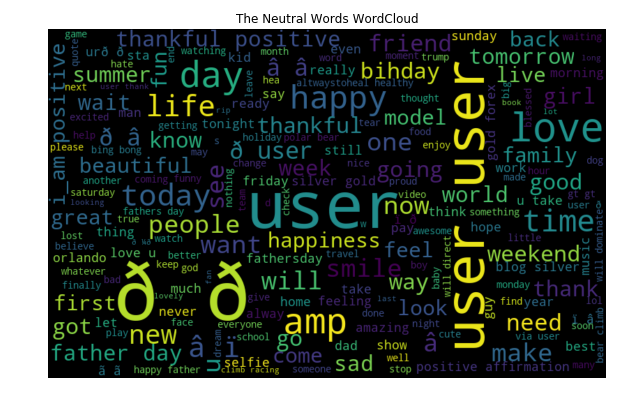
\includegraphics[width=5cm]{wordcloud2.png}
\caption{An example wordcloud output from our project\label{}}
\end{figure}

\section{Code Analysis and Outputs}

\subsubsection{ Data and Head}

All group members opened the csv files from the location on their computer, they used jupyter as an ide and zoom as a communication tool. Fatma  printed the head and the first 10 columns train part of the data, and Gizem printed the test part.

By pd.read csv (), the file is read by entering the datasets inside.

\begin{lstlisting}[language=Python, caption= data]
train = pd.read_csv(r'C:\Users\pesen\OneDrive\Desktop\Twitter-Sentiment-Analysis-master\train_tweet.csv')
test = pd.read_csv(r'C:\Users\pesen\OneDrive\Desktop\Twitter-Sentiment-Analysis-master\test_tweets.csv')
\end{lstlisting}

\\

With \textbf{head ()}, data belonging to a few lines is taken from the dataset and displayed on the screen. The desired number can be written here and the data can be drawn. For example, head (10) is drawn the first 10 lines.

\begin{lstlisting}[language=Python, caption= head]
train.head()
test.head()
\end{lstlisting}



\begin{figure}[ht!]
\centering
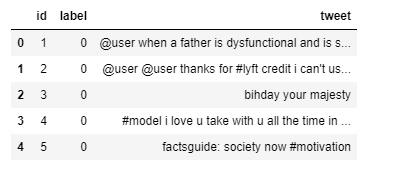
\includegraphics[width=9cm]{trainhead.png}
\caption{ Train head output\label{}}
\end{figure}

\begin{figure}[ht!]
\centering
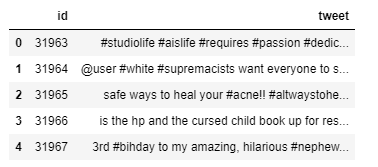
\includegraphics[width=9cm]{testhead.png}
\caption{Test head output \label{}}
\end{figure}

\subsubsection{Check Data With Isnull Method}

\textbf{isnull (). Any ()} method, Fatma suggested to check if there is a gap in the data with the isnull method , we checked if there is a gap and got a false output and continued our way with the result we got from this output. 


\begin{lstlisting}[language=Python, caption= isnull]
train.isnull().any() #Checked with isnull() method and it return false
test.isnull().any()
\end{lstlisting}

\begin{figure}[ht!]
\centering
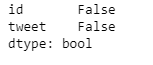
\includegraphics[width=5cm]{isnull.png}
\caption{There is no null values \label{}}
\end{figure}
.\\
\subsubsection{Negative and Positive Words}

Gizem looked at the examples and compared the tweets as 1 and 0 in binaries . With this line of code, we assigned the label value to 0 for negative words. We assigned a value of 1 to the label, which is positive. Thus, we have defined it as \textbf{binary}.

\begin{lstlisting}[language=Python, caption= label 0]
# to check the negative comments on the train set
train[train['label'] == 0].head(10)
\end{lstlisting}



\begin{figure}[ht!]
\centering
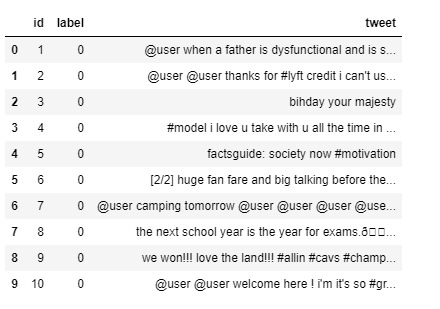
\includegraphics[width=10cm]{label0.png}
\caption{Label negative\label{}}
\end{figure}

Positive and negative results were visualized. (Plot is used for visualization.)
You can see clearly negative tweets are more than positive tweets with this graph.

\begin{lstlisting}[language=Python, caption=  0 and 1]
#We can see clearly negative comments are more than positive comments
train['label'].value_counts().plot.bar(color = 'pink', figsize = (6, 4)) 
\end{lstlisting}

\begin{figure}[ht!]
\centering
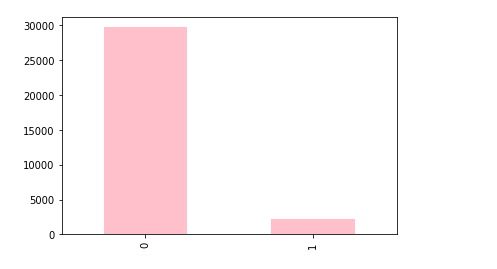
\includegraphics[width=10cm]{1and0.png}
\caption{ Comparing positive and negative tweets \label{}}
\end{figure}
.\\\\\\\\\\\\\\\\\
\subsubsection{Train and Test Data}

Fatma  compared her train and test data with the graph using her favorite colors of orange and pink. we stated that there is more train data from here.

\begin{lstlisting}[language=Python, caption= label 0]
# adding a column to represent the length of the tweet

train['len'] = train['tweet'].str.len()
test['len'] = test['tweet'].str.len()

train.head(10)
\end{lstlisting}


\begin{figure}[ht!]
\centering
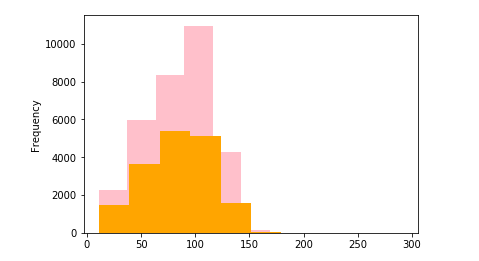
\includegraphics[width=12cm]{trainandtest.png}
\caption{Train and Test \label{}}
\end{figure}
.\\
\subsubsection{Length}
Gizem  added the data column as we needed the length of the words.

\begin{lstlisting}[language=Python, caption= label 0]
# adding a column to represent the length of the tweet

train['len'] = train['tweet'].str.len()
test['len'] = test['tweet'].str.len()

train.head(10)
\end{lstlisting}


\begin{figure}[ht!]
\centering
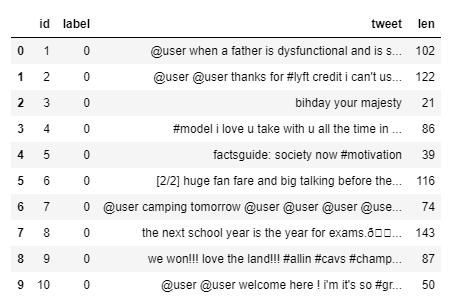
\includegraphics[width=8cm]{len.png}
\caption{Adding lenght \label{}}
\end{figure}


\subsubsection{Group Data}

Gizem grouped them as negative, positive tweets. With methods, also adding a column to represent the length of the tweet.
train.groupby ('label'). With the describe () method, we grouped negative and positive labels (labels defined as 0 and 1) in the train dataset and displayed them in a single table.

\begin{lstlisting}[language=Python, caption= group]
train.groupby('label').describe()
\end{lstlisting}


\begin{figure}[ht!]
\centering
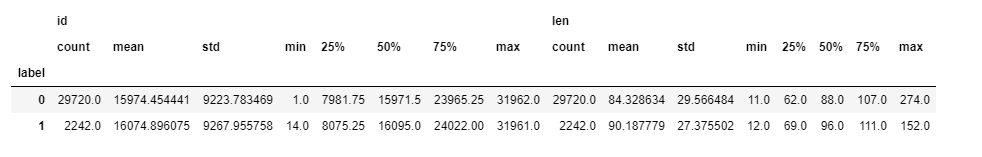
\includegraphics[width=15cm]{group.png}
\caption{Groupby \label{}}
\end{figure}

\subsubsection{Variation of Lenght}
Fatma  plotted the variation of length and found the relationship between frequency and length. The variety of the train dataset was shown with the methods.
\begin{lstlisting}[language=Python, caption= group]
train.groupby('len').mean()['label'].plot.hist(color = 'black', figsize = (6, 4),)
plt.title('variation of length')
plt.xlabel('Length')
plt.show()
\end{lstlisting}

\begin{figure}[ht!]
\centering
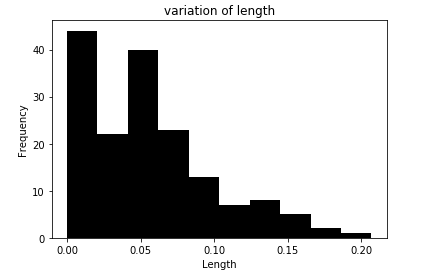
\includegraphics[width=10cm]{varlen.png}
\caption{Variation of lenght \label{}}
\end{figure}
\subsubsection{Most Frequently Occuring Words}

Both group members did the import and plotting of the Countvectorizer part together, and they had difficulty in this process.The frequency of the words in English was calculated using CountVectorizer from the Sklearn library, and the following graphic was created in order from high to low.


\begin{lstlisting}[language=Python, caption= group]
from sklearn.feature_extraction.text import CountVectorizer
count_vector = CountVectorizer(stop_words = 'english') #
words = count_vector.fit_transform(train.tweet)
sum_words = words.sum(axis=0)

words_frequency = [(word, sum_words[0, i]) for word, i in count_vector.vocabulary_.items()]
#çoktan aza giden sort edildi.
words_frequency = sorted(words_frequency, key = lambda x: x[1], reverse = True)
\end{lstlisting}
\\\\\\

\begin{figure}[ht!]
\centering
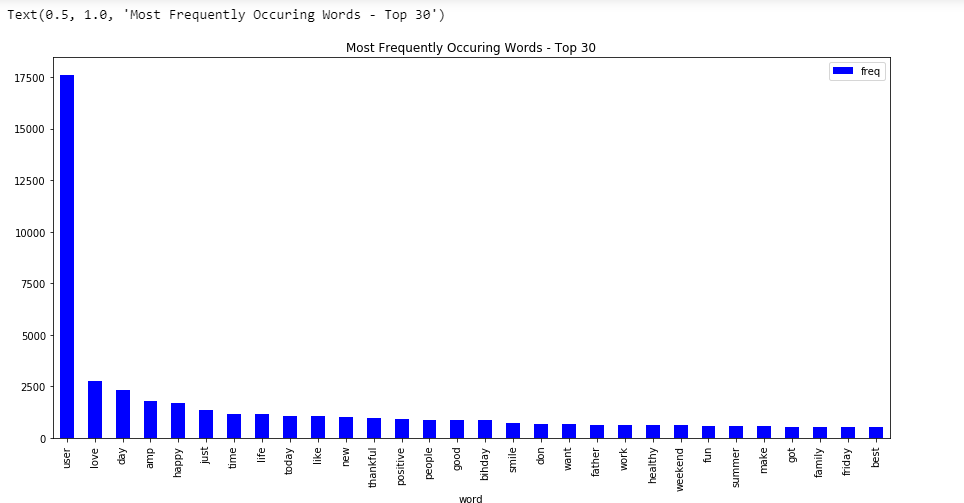
\includegraphics[width=18cm]{mostfreqword.png}
\caption{ \label{}}
\end{figure}


\section{Predictions}


\subsection{StandardScaler}
Most machine learning algorithms use the Euclidean formula, which measures the distance between two data points, one of the distance metrics, in their calculations. To ensure that all values contribute equally, the values must be brought to the same unit. The data, which varies in terms of size, will increase the variance and will not have an equal effect in distance calculations, as they will outweigh the low-value features in weight calculations. Data is scaled by feature standardization or Z-score normalization method. For this process, StandardScaler method of sklearn.preprocessing library is imported and used in python.

\subsection{RandomForestClassifier}


The Random Forest algorithm can be used in both classification and regression problems such as decision trees. Working logic creates more than one decision tree. When it will produce a result, the average value in these decision trees is taken and the result is produced.

\subsubsection{RandomForestClassifier Code Analysis}

we first included the libraries required for classification.

\begin{lstlisting}[language=Python, caption= RandomForestClassifier]
from sklearn.ensemble import RandomForestClassifier
from sklearn.metrics import confusion_matrix
from sklearn.metrics import f1_score
\end{lstlisting}

Then we assign the RandomForestClassifier() classification to the variable named model. And in the other classification methods we have made, we define the model variable and assign the classification methods to the model

\begin{lstlisting}[language=Python, caption= model]
model = RandomForestClassifier()
\end{lstlisting}

With the model fit () method, the information contained in the datasets is retrieved or in other words, the information is kept.

\begin{lstlisting}[language=Python, caption= model.fit]
model.fit(x_train, y_train)
\end{lstlisting}

We get predictions about the test data using the model.predict () function. Here we compare the basic accuracy values for the x valid sample with the predictions in our model.

\begin{lstlisting}[language=Python, caption= prediction]
y_pred = model.predict(x_valid)
\end{lstlisting}

We did print to print model.score on the screen.

\begin{lstlisting}[language=Python, caption= prediction]
print("Training Accuracy :", model.score(x_train, y_train))
print("Validation Accuracy :", model.score(x_valid, y_valid))

\end{lstlisting}

calculating the f1 score for the validation set

\begin{lstlisting}[language=Python, caption= prediction]
print("F1 score :", f1_score(y_valid, y_pred))
\end{lstlisting}

The confusion matrix allows us to compare test data with predicted values and measure the performance of our model.
TP (True Positive) and TN (True Negative) values give the correct number of values.
FP (False Positive) and FN (False Negative) values give the number of false values.
The ratio of the number of correct values to all the number of values indicates the Correct Prediction Ratio.
The ratio of the number of false values to all the number of values indicates the False Prediction Rate.

\begin{lstlisting}[language=Python, caption= cm]
cm = confusion_matrix(y_valid, y_pred)
print(cm)

\end{lstlisting}
\\\\
\textbf{Output}

\begin{lstlisting}[language=Python, caption= Accuracy ]
Training Accuracy : 0.9944933461265696
Validation Accuracy : 0.9481917156801402
F1 score : 0.5775510204081632
\end{lstlisting}

\subsection{LogisticRegression}
Logistic Regression is a regression method for classification. It is used to classify categorical or numerical data. It works only if the dependent variable, ie the result, can take 2 different values. (Yes / No, Male / Female, Fat / Thin etc.)
\\\\
\textbf{Output}

\begin{lstlisting}[language=Python, caption= Accuracy ]
Training Accuracy : 0.984773267698469
Validation Accuracy : 0.9410586910274058
f1 score : 0.5915004336513443
\end{lstlisting}

\subsection{DecisionTreeClassifier}
The decision tree is a recursively process, as the name suggests, a tree structure is used. A tree structure is created by starting with a single node and branching into new results. When the algorithm runs, the entered value moves on a certain path by looking at the nodes and gives a result.
There are 3 types of knots.

\begin{enumerate}
\item Chance Node: It is indicated with a circle. Indicates multiple possible paths.
\item Decision Node: It is indicated with a rectangle. Indicates that a decision will be made.
\item End Node: It is indicated with a triangle. Indicates a result.
\end{enumerate}

\\\\
\textbf{Output}

\begin{lstlisting}[language=Python, caption= Accuracy ]
Training Accuracy : 0.9991656585040257
Validation Accuracy : 0.9325491177574772
f1 score : 0.5404944586530265
\end{lstlisting}



\subsection{SVC}

It can classify or regress data by making use of gaps between data. However, it is generally used for classification. It can be applied in clustering or outlier detection. Basically, it allows us to distinguish between data with the help of SVM vectors.
\\\\
\textbf{Output}

\begin{lstlisting}[language=Python, caption= Accuracy ]
Training Accuracy : 0.978181969880272
Validation Accuracy : 0.9521962207483419
f1 score : 0.4986876640419947
\end{lstlisting}





\subsection{SGDClassifier}
\\\\
\textbf{Output}

\begin{lstlisting}[language=Python, caption= Accuracy ]
Training Accuracy : 0.9820199407617538
Validation Accuracy : 0.9499436866474784
f1 score : 0.5815899581589958
\end{lstlisting}

 

\section{Conclusion}


We tried to explain the libraries and classification methods we used while doing this project homework step by step above, and we supported the results of these analyzes with screenshots.

Since the scores we obtain from the classification methods we use are usually very close to 1 (between 0.94-0.98), it shows that the classification methods we use are the right choice for the data set we analyze. Sgd Classifier and Decision Tree Classifier calculated by Fatma ;   RandomForestClassifier and SVC calculated by Gizem. The best prediction is 0.9991656585040257 with  Decision Tree Classifier.
In the few articles we have read, your score for your data set close to 1 has been written as proof that analyzing the data you have is the right choice.
Taking this as a reference, we think our choices are correct.





\section{References }
\\
\textbf{[]} \url{https://www.veribilimiokulu.com/kernel-support-vector-machine-svm-ile-siniflandirma-python-ile-ornek-uygulama/}
\\
\textbf{[]}  \url{https://www.websitehostingrating.com/tr/twitter-statistics/}
\\
 \textbf{[]} \url{https://ai.yemreak.com/makine-ogrenimi/scikit-learn}



\end{document}

